\subsection{Indkøbsliste}
En indkøbsliste kommer til verden ved, at man i husstanden beslutter sig for at benytte en eller anden form for huskeliste for ting, der skal handles ind. Dette kan være i form af et papir, der ligger et fast sted på bordet eller hænger på opslagstavlen. Denne initierende hændelse kaldes \textit{indkøbsliste oprettet}. Se \figref{fig:indkoebsliste-adfaerd}.

Så længe indkøbslisten ligger på bordet eller et andet sted, kan mange personer komme forbi og tilføje eller fjerne varer på den. Denne tilstand kaldes for \textit{redigeres}. I denne tilstand er det muligt for alle, der kan komme til denne indkøbsliste, at tilføje eller fjerne de varer, der skal handles ind. Man kan \fx fjerne en vare ved at slå en streg over den og give et klart signal om, at denne ikke skal købes. Disse to hændelser hedder \textit{vare fjernet} og \textit{vare tilføjet}. Personen, der tilføjer tekst til indkøbslistene, er herre over, om der skal stå en ingrediens, der består af en mængde, en enhed og en råvare (\fx 1 ltr skummetmælk) eller der blot skal stå råvaren (\fx skummetmælk).

Indkøbslisten kan også indeholde bemærkninger, såsom ``hvis det er på tilbud''. Denne bemærkning kan selvfølgelig også fjernes igen på samme måde som en vare kan fjernes. Disse bemærkninger tilhører en eller flere varer på indkøbslisten, og derfor er hændelsen den samme som ved tilføjelse eller fjernelse af en vare.

Når en person beslutter sig for at tage indkøbslisten med på indkøb, anses indkøbslisten for at være færdig. Det er nu ikke længere muligt at redigere i indkøbslisten, og den afsluttende hændelse indtræffer. 

Ude i supermarkedet kan man købe mange forskellige råvarer. Vi ønsker ikke at overvåge, hvor meget folk har af en ingrediens, og benytter derfor istedet objektet råvare, der ikke indeholder nogen mængde eller enhed. Denne beslutning er taget på baggrund af møde 2 med vores informanter.\todo{Argumenter lidt bedre for valget.}

\begin{figure}[H]
	\centering
	\scalebox{0.8}{
		\subsection{Indkøbsliste}
\label{subsec:brug-indkoebsliste}

Ud over muligheden for at tilføje opskrifternes ingredienser til indkøbslisten, så kan man også tilføje almindelig tekst til, så det er muligt at lave en indkøbsliste, der indeholder andet end ingredienser til madlavningen. Så man kan skrive andre varer på, som man kan købe med fra \fx supermarkedet. Systemets indkøbsliste kan ses i \figref{fig:overblik-indkoebsliste}.

\begin{figure}[H]
	\centering
	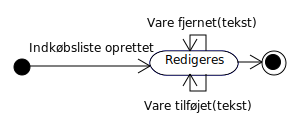
\includegraphics[scale=1]{billeder/foodl/thumbnails/indkoebsliste.png}
	\capt{Denne figur har til formål at give et overblik over systemets indkøbsliste.}
	\label{fig:overblik-indkoebsliste}
\end{figure}

Brugeren har mulighed for at tilføje varer i feltet ``tilføj til indkøbsliste'' og trykke på ``tilføj'' i bunden af siden. Der er mulighed for at slette alle varer fra indkøbslisten, ved at trykke på knappen ``slet alt'' i øverste højre hjørne af indkøbslisten, og ligeledes at slette enkelte varer, ved at trykke på de små gule krydser ud for alle varerne. Derudover er der implementeret en knap, til at udskrive indkøbslisten, som vi naturligvis kalder for ``udskriv''.

Hvis brugeren ikke er logget ind, vil de se i øverste højre hjørne af \figref{fig:overblik-indkoebsliste} (under sidehovedet) en boks, som informerer brugeren om, at man skal være logget ind for at systemet skal være i stand til at gemme indkøbslisten og favoritter. Oprettelse af bruger og indlogning bliver beskrevet nærmere i \secref{subsec:brug-opret}.
}
		\capt{Tilstandsdiagram for klassen indkøbsliste. De afrundede rektangulære bokse med tekst, skal anses som tilstande, som klassen kan have. De pile, der fører til en tilstand, skal anses som hændelser, som kan være skyld i et tilstandsskift. I dette tilfælde har klassen én tilstand (redigeres) og en afsluttende hændelse, der fører klassen ud i en sluttilstand (den sorte prik i den sorte cirkel).}
		\label{fig:indkoebsliste-adfaerd}
\end{figure}